
\section{Accelerators and Detectors: Basic Principles}
%%\begin{itemize}
%%    \item from the start; Magnetic rigidity(?)
%%    \item acceleration
%%    \item magnetic focussing, FODO, dipole, quadropole
%%    \item detector basics, (relevant) detector types, basic of bethe bloch
%%    \item luminosity calculations, bunch and crossings
%%    \item cross section
%%    \item Limiting factors
%%\end{itemize}


\section{The Large Hadron Collider}
The Large Hadron Collider (LHC) is a modern proton-proton synchrotron located at the CERN complex, outside of Meyrin, Switzerland. At a circumference of approximately 27km the LHC is currently the largest particle accelerator on the planet, and similarly produces the highest centre-of-mass energies for $pp$ collisions, reaching $\sqrt{s}=13\text{TeV}$. The LHC was constructed from 1998-2008 in the tunnel previously occupied by the Large Electron-Positron Collider (LEP). It extends from from the CERN site, across the French border towards the Jura Mountains and round returning through Geneve and Meyrin. It is positioned on a plane inclined at $1.41\%$ between 45-175 metres underground, a measure to protect both the experimental recordings from a large fraction of cosmic ray interference and the surface from any hazardous emissions from either the particle collisions or the synchrotron radiation.

The LHC is supported by a number of smaller accelerator systems designed to provide proton bunches of the correct spacing and energy, these are visible in figure \ref{fig:accel_complex}. The acceleration process begins with the injection of Hydrogen anions ($\text{H}^{-}$) into LINAC\footnote{This was LINAC 2 until 2020, reaching $50\text{MeV}$. During Long Shutdown 2 (LS2) this was obsolesced by LINAC 4}, which provides an acceleration to energies of $160\text{MeV}$ before the beam is passed on the Proton Synchrotron Booster (PSB)\footnote{\href{https://cds.cern.ch/journal/CERNBulletin/2016/32/News\%20Articles/2201549?ln=en}{idk psb}}. This continuous beam from LINAC is stripped of electrons and split consecutively amongst the four PSB rings, accelerated to $1.4\text{GeV}$, and injected into the Proton Synchrotron (PS). PS produces bunches spaced by $25\text{ns}$, accelerates these to $25\text{GeV}$, and passes them over to the Super Proton Synchrotron (SPS) for the final energy increase up to $450\text{GeV}$.
\begin{figure}[!h]
    \centering
    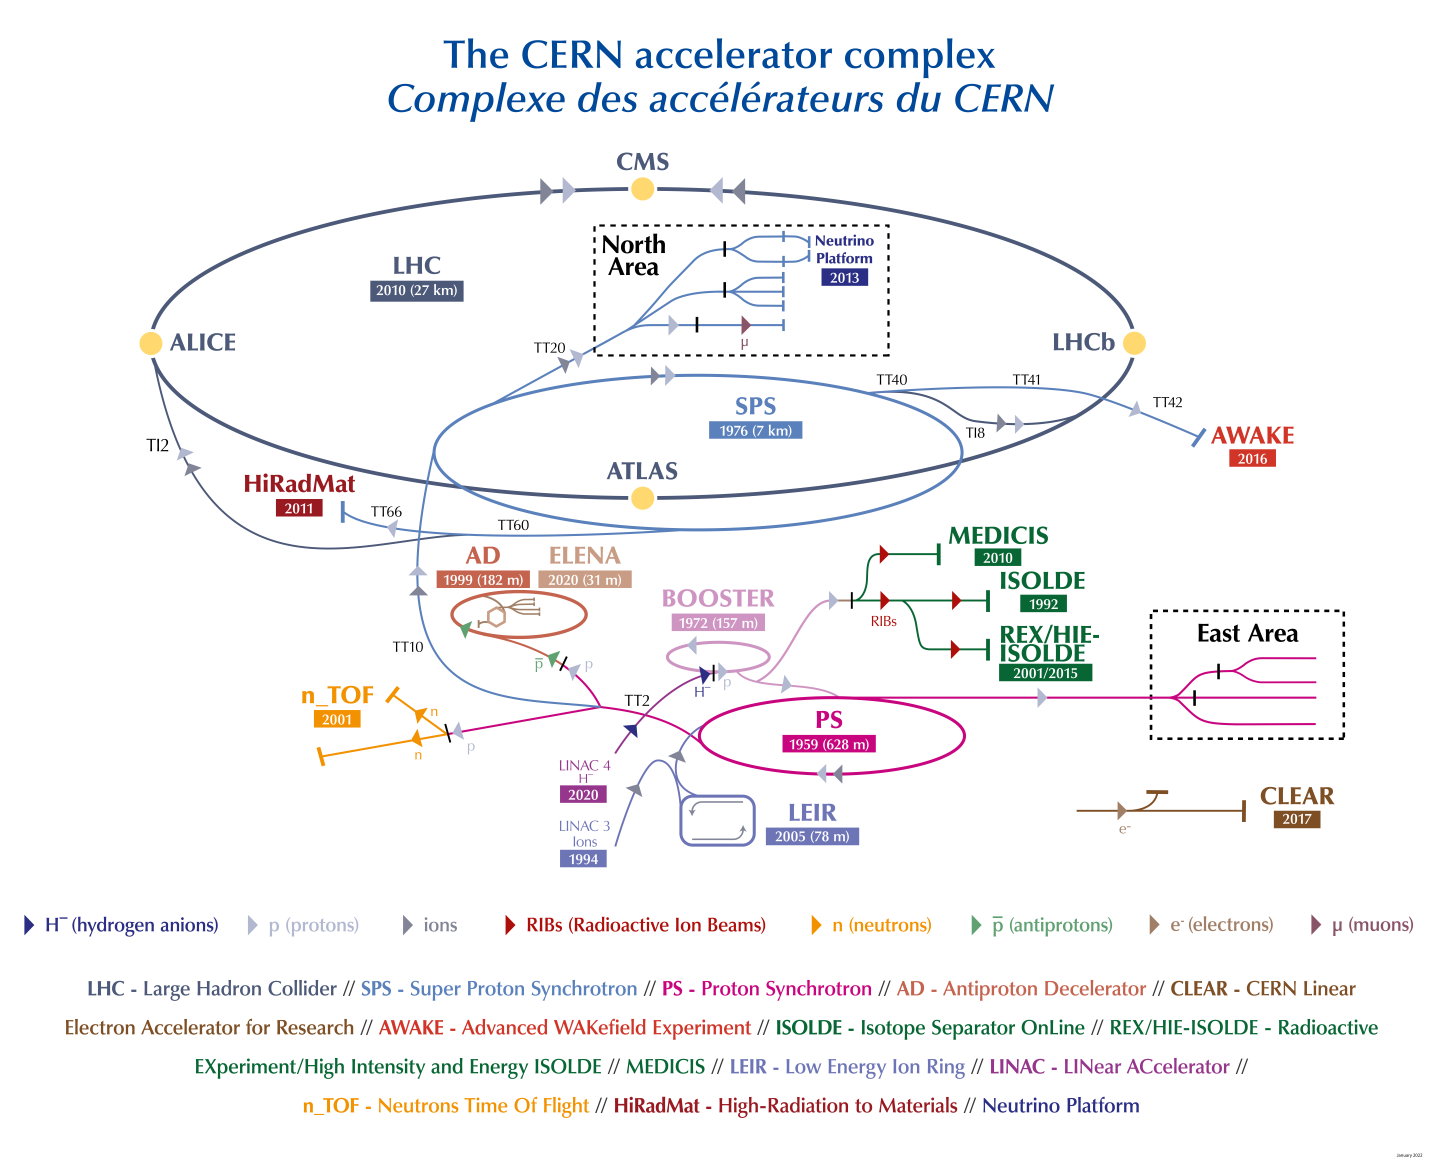
\includegraphics[]{figures/lhc_and_atlas/CCC-v2022.png}
    \caption{CERN Accelerator Complex schematic \cite{lopienska2022}. }
    \label{fig:accel_complex}
\end{figure}
Bunches inserted from SPS into the the LHC are brought from $450\text{GeV}$ up to $6.8\text{TeV}$ over a timespan of approximately 20 minutes. This is driven by the 16 RF cavities around the LHC ring, oscillating at $400\text{MHz}$ each providing up to $2\text{MV}$ of acceleration. The LHC beampipe is a dual-core design allowing bunches to travel in different directions allowing the CoM to coincide with the lab frame of a detector. For a single turn through the LHC, a proton bunch will pass through the magnetic field of 1232 superconducting dipole magnets. The magnets are of Niobium-titanite construction, are held at 1.9K, and produce a field of $\sim8.3\text{T}$. In order to amplify luminosity at the interaction point a focussing effect is produced by the 474 quadropole magnets, arranged into FODO lattices positioned throughtout the circumference.

There are 8 experiments that are part of the LHC, 4 of which are positioned around the circumference. These 4 are ATLAS, LHCb, CMS, and ALICE, located at points 1, 8, 5, and 2, respectively. These experiments are collectively engaged in Run 3 of the LHC. After commissioning and a magnet quench incident in 2008, the LHC entered full operation on 20 November 2009 with first collisions at $7\text{TeV}$ occuring on 30 March 2010. Run 1 concluded in early 2013, delivering a total integrated luminosity of $22.8\text{fb}^{-1}$. Run 2 began in 2015 and extended into 2018, raising the collision energy to $13\text{TeV}$, and delivering a total of $140\text{fb}^{-1}$. After LS2\footnote{2018-2022} and the upgrades to both the LHC and detectors associated with this, the LHC began Run 3 operations with an increase in the collision energy, again, to $13.6\text{TeV}$, and is currently ongoing in 2024. After Run 3, the LHC enters Long Shutdown 3 (LS3) for a series of upgrades to prepare for the HL-LHC phase where there is a roughly eight-fold increase in peak luminosity planned, and the total integrated luminosity over the HL-LHC period from Run 4 to the end of Run 6 planned in 2038 will be $4000\text{fb}^{-1}$.


%% https://twiki.cern.ch/twiki/bin/view/AtlasPublic/LuminosityPublicResults#Integrated_luminosity_summary_pl

% h##ttps://physics.stackexchange.com/questions/474122/how-is-a-proton-beam-separated-into-bunches-in-a-particle-accelerator
%%h##ttps://cds.cern.ch/record/446600/
%% ##"we must make sure that the particle always sees an accelerating voltage at the gap, so the RF frequency must always be an integer multiple (h) of the revolution frequency."
%% ##https://www.lhc-closer.es/taking_a_closer_look_at_lhc/0.buckets_and_bunches
%% https://home.cern/science/accelerators
%%https://cds.cern.ch/record/1982419/files/61-100%20Holzer.pdf


%%SPS, LHC, fills reaching an energy of 13.6TeV, 6.8TeV per beam
%%
%%Accelerated by RF Cavities oscillating at 400MHz
%%
%%
%%The LHC 'ring'
%%
%%Dual-core beampipe, common cryostat
%%1232 dipoles, Niobium-titanite construction, ~8.3T at 1.9K
%%474 Quadropoles
%%
%%The Focussing process is performed 



%Points to make
%\begin{itemize}
%    \item precise location x 
%    \item geometry, straight and curved sections 
%    \item points and active experiments x
%    \item full accelerator complex rundown, energies, etc x
%    \item run details peak luminosities x
%    \item upgrades and futures *
%    \item effects of high energies, pileup, etc x
%    \item bunch details, bunch grouping, injection etc x
%    \item cosmics and radiation protection x
%\end{itemize}





\section{The ATLAS Detector}
\subsection{Overview}
The ATLAS Detector[CITATION] as a general-purpose detector with cylindrical geometry and a forwards-backwards symmetry. It has nearly complete coverage, approaching $4\pi$, in solid angle around the interaction point (IP) which is located centrally within the detector layout. The detector is located at Point 1 on the LHC ring, approximately $100m$ below the surface, with the ATLAS control room and supporting infrastructure located directly above at the Meyrin site of CERN.
\begin{figure}[!h]
    \centering
    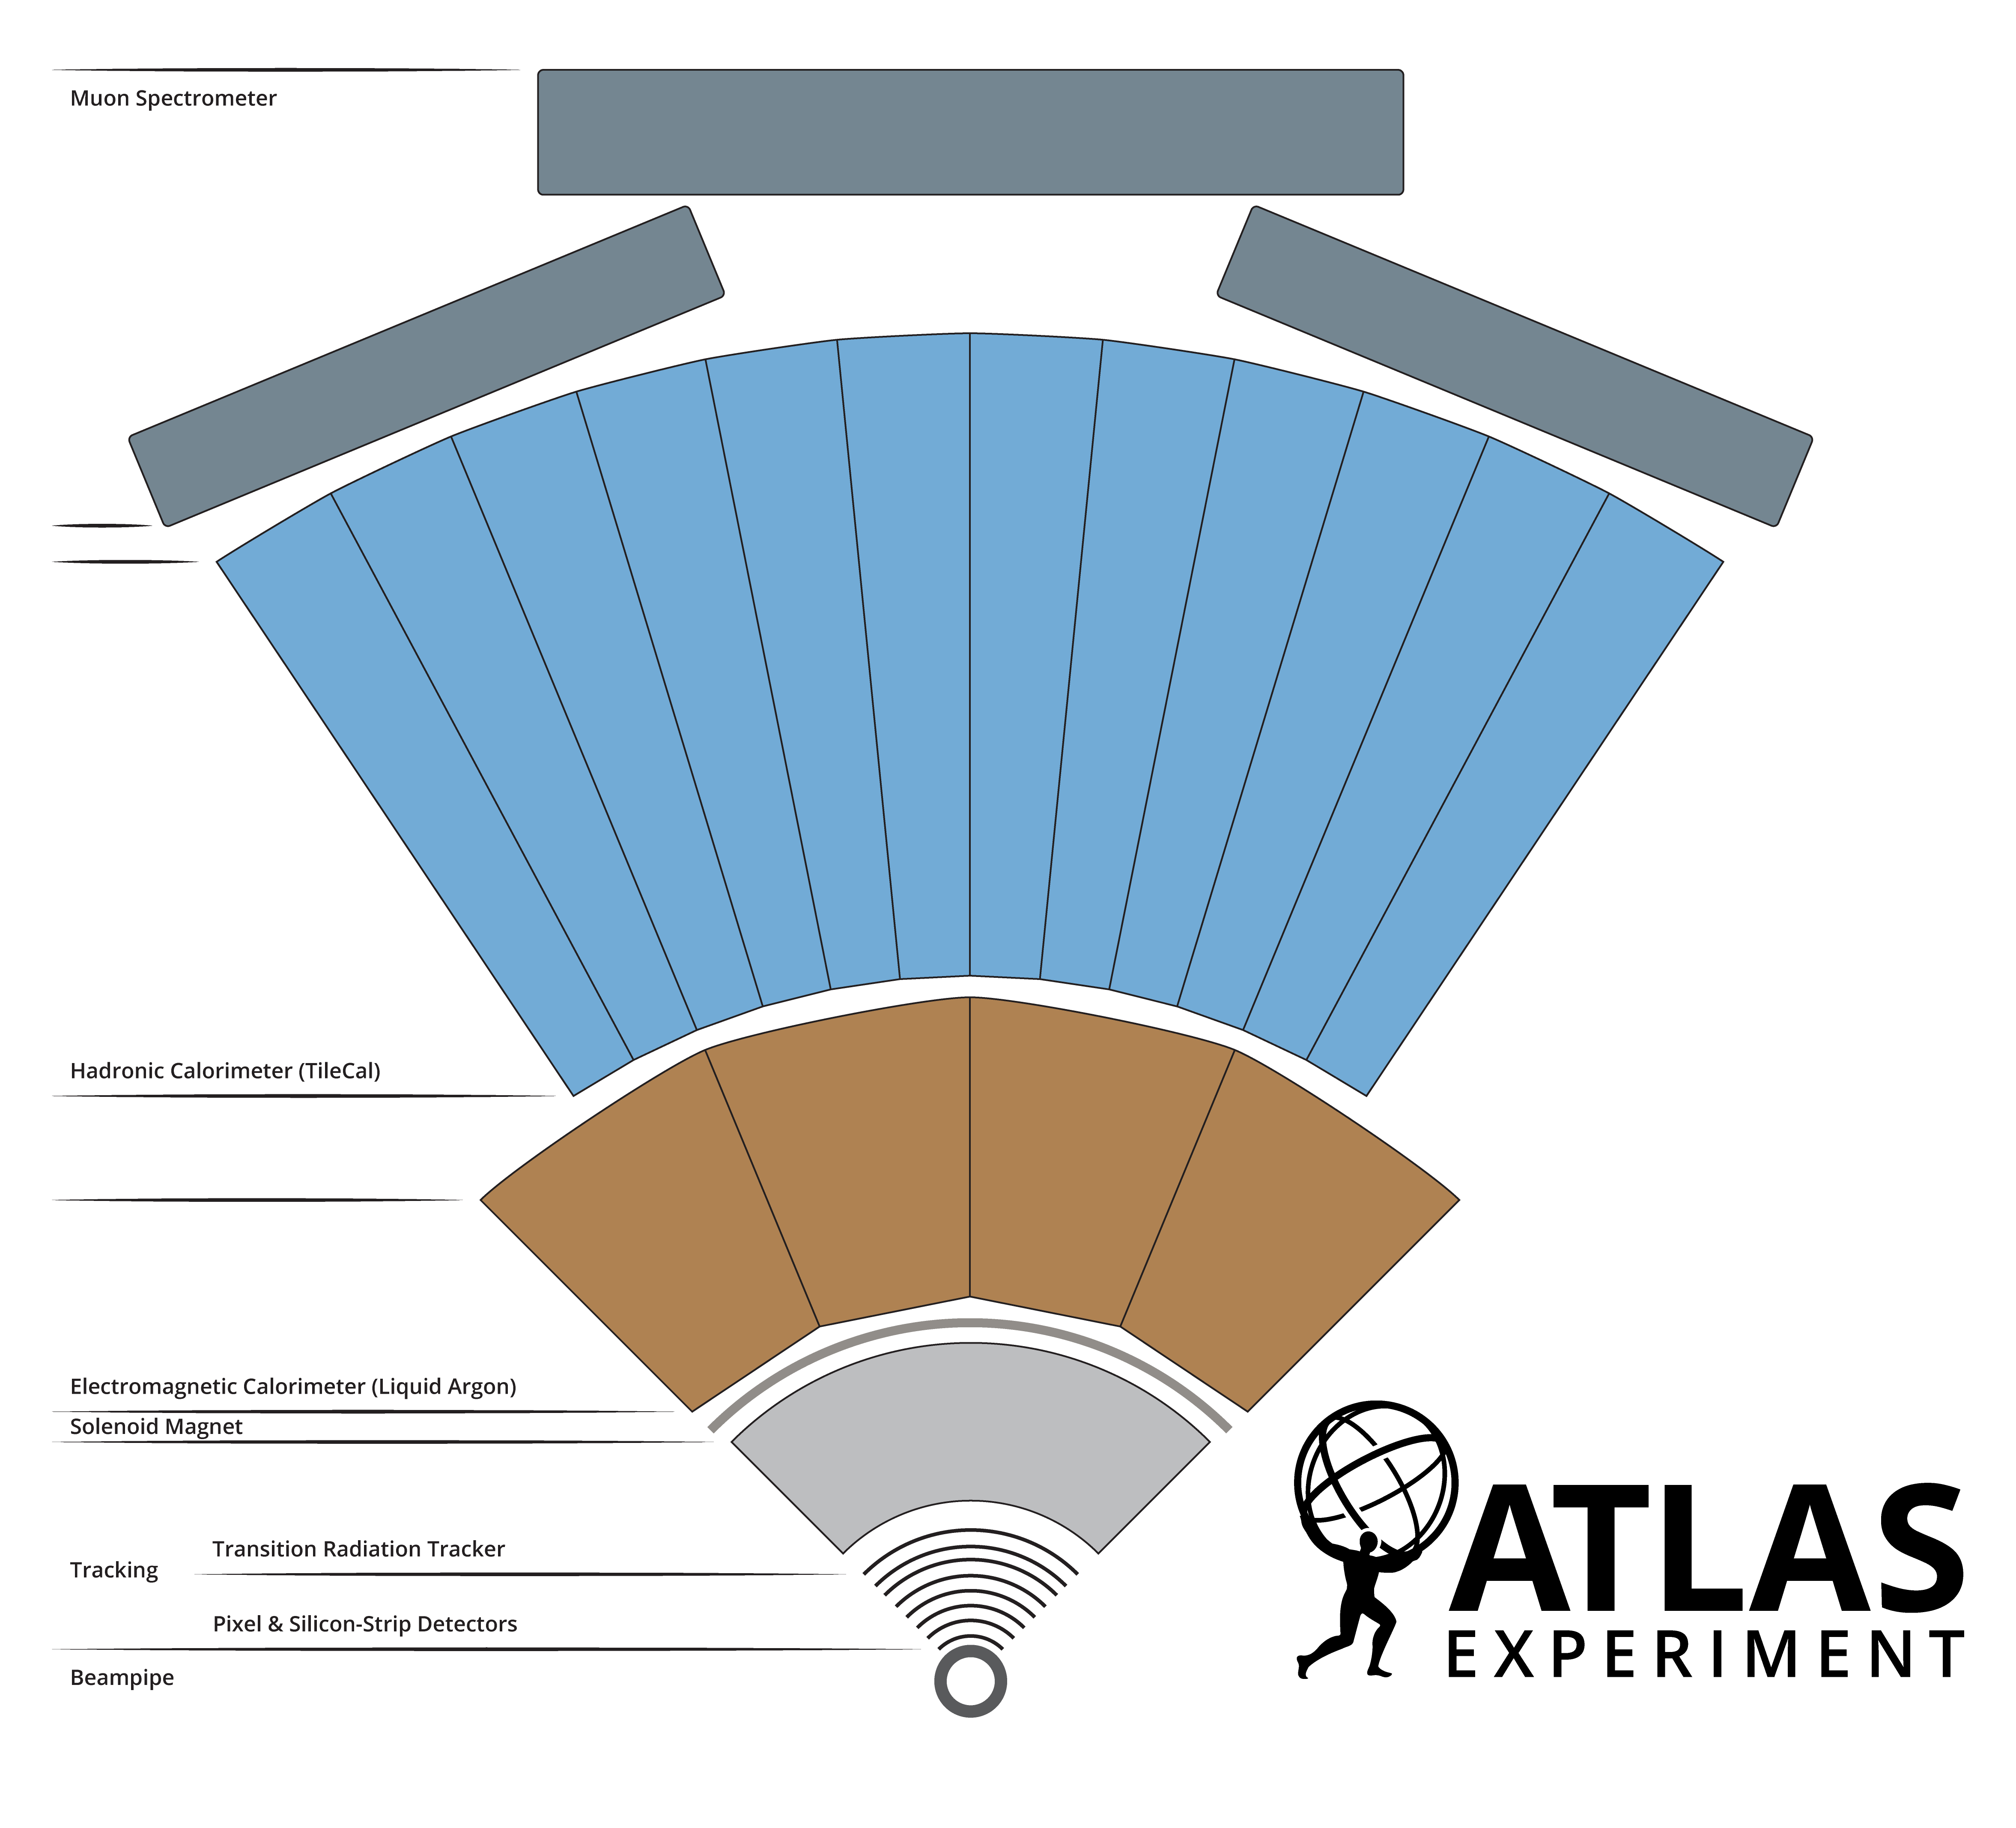
\includegraphics[width=\textwidth]{figures/lhc_and_atlas/ATLAS_DET_SLICE.png}
    \caption{Cross-Sectional slice of the ATLAS detector \cite{Mehlhase:2770815}. }
    \label{fig:detslice}
\end{figure}
There are a number of main subsystems within the ATLAS detector, a cross-section of the detector outlining their positions is shown in \ref{fig:detslice} . Starting centremost radially, closest to the interaction point there is the Inner Dectector (ID) comprised of the Pixel Detector, the Semi-Conductor Tracker (SCT), and the Transition Radiation Tracker (TRT). This is used to provide tracking information for all charged particles created in an event, a $pp$ collision. The ID is immersed in a solenoidal magnet, producing a 2T field to generate a curvature in charged particle paths. Outside of this, the calorimeter systems begin with the Electromagnetic Calorimeter (ECal). The ATLAS ECal is a LAr Calorimeter in both the Barrel and Endcap Regions, and is used for precision measurement of Electron and Photon signals. The Hadronic Calorimeter (HCal) systems follow the ECal, these are designed for the measurement of strongly interacting particles which traditionally pass through the ECal and form showers further out from the interaction point. Three main components form the HCal, the Tile Calorimeter (TileCal) in the barrel region, and LAr calorimeters form the detector setup. in the endcap and forward regions. Last in the sequence are the Muon Systems (MS), placed in the outermost region to collect muons that typically penetrate through the earlier stages of the detector, or any other charged particles that may leak from the other inner stages. The MS is constructed from two main components in the barrel.




%%\begin{itemize}
%%    \item Basic detector details.
%%    \item Some collaboration details.
%%    \item Location and control room.
%%    \item Sides.
%%    \item Support infrastructure.
%%\end{itemize}


\subsection{Coordinate system and common variables}
To perform physics analysis at a $pp$ experiement, several variables must be defined to accurately describe the physics objects that will be detected. The Cyclindrical geometry of ATLAS lends towards using a cylindrical coordinate system for analysing events and is defined from a cartesian system centered around the interaction point. The $x$-axis points towards the centre of the LHC ring, the $y$-axis directly upwards, and the $z$-axis along the beamline. The Azimuthal angle $\phi$ in this cylindrical system begins at the $x$-axis, and the polar angle $\theta$ at the $z$-axis.

\begin{itemize}
    \item \textbf{Energy $E$.} The energy of particles that are produced in reactions. This can be assessed as the particle with deposit energy into the calorimeter materials as it travels outwards from the interaction point.
    \item \textbf{Transverse Momentum $p_{T}$.} This is the component of a particle momentum in the plane transverse to the beam line. In ATLAS this is used in preference to overall momentum on the basis that it is a conserved variable and is more informative of the physics given the typical kinematic distribution of events that would be expected in a $pp$ collision of the nature at the LHC.
    \item \textbf{Invariant mass $m$.} Invariant mass can be used in the context of single particles or systems of them. Calculating the invariant mass of selected combinations of particles can yield information on the resonant particles within an event or interaction. This is typically calculated through combining information collected on the momentum and energy of a particle, or collecton of particles.
    \item \textbf{ Rapidity $y$, Pseudorapidity $\eta$, and Distance $\Delta R$.} These three variables help define a particle position after an interaction. Rapidity is an angular and relativistic measure of velocity, that can be used to define $$y = -\frac{1}{2} \ln{\frac{E+p_{z}}{E-{p_{z}}} }.$$ Beneficially, rapidity differences are lorentz-invariant. When the particle masses are far smaller than the energy the rapidity can be approximated to the pseudorapidity, a more easily calculable and purely angular variable defined as $$\eta = -\ln\tan{\frac{\theta}{2}}.$$ When combined with the azimuthal angle $\phi$, a lorentz-invariant distance measure appropriate for the cylindrical geometry can be defined; $$\Delta R = \sqrt{\Delta \eta^{2} + \Delta \phi^{2}}.$$
    \item \textbf{ Tracking Parameters $z_{0}$, $d_{0}$, and $\frac{q}{p}$ } When combined with the beamspot position, $\theta$ and $\phi$, these 5 variables are used to fully define a track in ATLAS. $z_{0}$ is the longitudinal impact parameter, measuring the closest approach of the track to the beamspot along the axis of the beam, $d_{0}$ distance of closest approach of a track to the beamline in transverse plane, and $\frac{q}{p}$ is the charge-momentum ratio of a reconstructed track.
    \item \textbf{ Transverse displacement $L_{xy}$, and lifetime $\tau$.} $L_{xy}$ is the transverse displacement of a point, typically the vertex of a particle decay, from the beamline. Due to the relativistic nature of particles and the fact $L_{xy}$ is not a variable natural to the rest frame of any decaying particle, it is preferable to use the pseudo-proper lifetime $\tau$ in many cases; $$ \tau = \frac{L_{xy}m_{parent}}{c\cdot p_{T}} $$



\end{itemize}
    
%%\begin{itemize}
%%    \item Rapidity and Pseudorapidity *
%%    \item Azimuthal, eta-phi space *
%%    \item impact parameters *
%%    \item Common kinematic and analysis variables*
%%\end{itemize}

\subsection{Inner Detector}

%% GOOD PIXEL REFERENCE RUN1 - https://cds.cern.ch/record/1262789/files/EurPhysJC.3FBE7E53d01.pdf
%% GOOD PIXEL REFERENCE RUN2 - https://cds.cern.ch/record/1985432/files/ATL-INDET-PROC-2015-001.pdf
%% GOOD PIXEL REFERENCE RUN3 - https://cds.cern.ch/record/2851225/files/ATL-INDET-PROC-2023-001.pdf
%% APPROVED PLOTS - https://twiki.cern.ch/twiki/bin/view/AtlasPublic/ApprovedPlotsATLASDetector#:~:text=ATLAS%20Run%2D3%20Detector%20Status%20(from%20May%202023),-Subdetector&text=The%20Pixel%20status%20includes%20the,to%20the%20number%20of%20cells.
The ATLAS Inner Detector (ID), the first detector subsystem, provides the backbone of tracking and vertexing information for events recorded during LHC runs. Starting at a radius of $3.3\text{cm}$ the detector extends out to $1.05\text{m}$ and is $6.2\text{m}$ long. Innermost to this system, $3.3\text{cm}$ from the beamline, is the pixel detector (PIX/IBL), consisting of 4 layers of pixel layers, the innermost Insertable B-Layer (IBL) was installed in 2014. The IBL has a smaller pixel size, of $50\times250\mu\text{m}$, than the other pixel layers with $50\times400\mu\text{m}$, and was inserted to increase the tracking resolution of the ID. PIX/IBL provides $92$ million readout channels, $12$ million from the IBL alone, with a total $1.9\text{m}^{2}$ of silicon area.

%% GOOD SCT Run 2 - https://iopscience.iop.org/article/10.1088/1748-0221/9/08/P08009/pdf
%% SCT MODULES https://www.sciencedirect.com/science/article/abs/pii/S0168900207007644?via%3Dihub 
%% END MODULES https://www.sciencedirect.com/science/article/abs/pii/S0168900207003270?via%3Dihub
%% Barrel modules - https://cds.cern.ch/record/974073/files/indet-pub-2006-005.pdf
%% MORE - https://www.sciencedirect.com/science/article/pii/S0168900207007644?ref=cra_js_challenge&fr=RR-1

The second subsystem of the ID is the SemiConductor Tracker (SCT). As of Run 3 this is operating with 6.3 million readout channels consisting of silicon 'micro-strips', in 4088 modules arranged across 4 barrel layers (2112 modules) and 18 endcap disks, nine each side ($988\times 2$), covering an area of $60\text{m}^{2}$. Detector planes are offset by $40\text{mrad}$ to assist in providing a readout accuracy as tight as $25\mu\text{m}$. All modules in the barrel region are identical, they consist of four sensors paired off and connected back to back. Across the four sensors in a module there are 3072 readout strips (768 per sensor), pitched identically at $80\mu\text{m}$. The endcap modules have a variable micro-strip pitch dependent on their position as a function of their wedge-like geometry, though still have 768 readout strips per sensor.

%% TRT 1 - https://cds.cern.ch/record/2139567/files/ATL-INDET-PROC-2016-001.pdf
The outermost section of the ID consists of the Transition Radiation Tracker (TRT). This is constructed from 300,000 thin-walled drift tubes of $4\text{mm}$ diameter with a total volume of $12\text{m}^{3}$. In the barrel region the straws are aligned parallel to the beam axis and extend from 560mm to 1080mm in radius. In the endcap region, the straws are alinged perperndicularly. Particle identification is performed with a combination of ionisation-loss curve analyisis - CHECK, and using the probability of certain particles to produce readout pulses in the TRT that cross certain low and high $\text{eV}$ thresholds, LT and HT respectively. The HT threshold for example is used for electrion-pion discrimination. 

\subsection{Calorimetry}
The ATLAS calorimeter system is composed of two detector types, each type predominantly assigned to the two different tasks of Electromagnetic (ECal) and Hadronic (HCal) energy measurements. The LAr Calorimeter system consists of four components, the LAr Forward Calorimeter (FCal) for both ECal and HCal purposes, the LAr hadronic end-cap (HEC), the LAr electromagnetic end-cap (EMEC), and the LAr electromagnetic barrel. HCal in the barrel region is perormed by the Tile Calorimeter (TileCal).

\subsubsection{EM Calorimetry}


%%* first radially from the centre
%%6.2 metres long
%%2.1 metres in diameter
%%thickness?
%hits in this region of the detector produce the seeds for reconstructing tracks and vertices
%The ID is the backbone of tracking and vertexing in atlas

%% Digitisation in sensors often done with 'Time Over Threshold' this is turned into 1's 

%%There's 3 main layers, 
%%
%%the pixel detector,
%%    four layers
%%    92m channels
%%    1.9m2 of silicon area
%%    15kW of power consumption
%%    innermost layer IBL -> 3.3cm from the beamline, installed in 2014 to enhance tracking
%%    pixels are 50x250um in the IBL
%%    pixels are 50x400um on the outer 
%%    the four barrel layers have 1744 modules
%%    the three end-cap discs have 288 modules
%%
%%SCT - SemiConductor Tracker
%%    silicon strip detector, 6.3 million channels
%%    4088 barrel modules on 4 cylinder layers
%%    4 detector wafers with 768 strips
%%    80um pitch
%%    Endcap is two sets of 9 disks
%%        trapezoidal detector wafers with 56.9-90.4um pitch
%%    2 planes are offset by 40mrad, this gives stereo


%%TRT - thin-walled drift tubes
%%    300,000 of them, 4mm in diameter
%%    12m3 of volume
%%    50,000 straws in barrel
%%    the rest are in the endcaps
%%    this gives information on particle type
%%
%%    
%%How do we ID in the inner detector? -> Ionisation-loss curves -> offline problem though no?
%%
%%
%%the entire inner detector will be replaced by the all-silicon ITk -> extension of up to 9 hits for most particles in run 4, coverage up to eta 4 - https://indico.cern.ch/event/803258/contributions/3582845/attachments/1962390/3265284/259-Buttar-ATLASPixelsOverview-v3.pdf
%%
%%add both those Inner detector diagrams

%%\subsection{Calorimetry}
%%\subsubsection{Electromagnet Calormiter}
%%\subsubsection{Hadronic Calorimeter}
%%\subsection{Muon Systems}
%%\begin{itemize}
%%    \item I don't even know yet
%%\end{itemize}
%%\subsection{Magnetic Setup}
%%\begin{itemize}
%%    \item The central solenoidal magnet
%%    \item The toroidal magnets
%%    \item Magnetic diagram
%%\end{itemize}
%%
%%\subsection{Trigger and Data Acquisition}
%%\begin{itemize}
%%    \item L1 and HLT etc
%%    \item Online trigger system - CTP etc
%%    \item offline reprocessing
%%\end{itemize}
